51. \begin{figure}[ht!]
\center{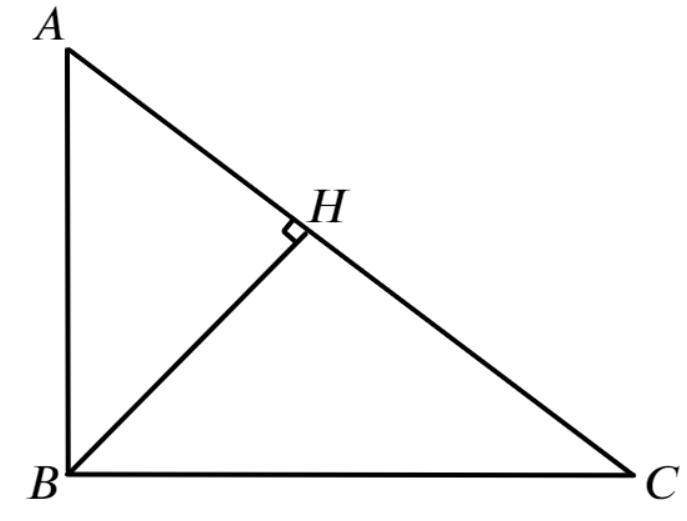
\includegraphics[scale=0.35]{g8-51.png}}
\end{figure}\\
Пусть катеты прямоугольного треугольник равны $3x$ и $4x,$ тогда по теореме Пифагора $9x^2+16x^2=2500,\ x^2=100,\ x=10.$ Тогда площадь треугольника $ABC$ с одной стороны равна $\cfrac{1}{2}\cdot30\cdot40=600,$ а с другой стороны равна $\cfrac{1}{2}BH\cdot50=25BH,$ значит $BH=600:25=24.$ По теореме Пифагора для треугольника $ABH$ имеем $AH=\sqrt{900-576}=18,$ тогда $HC=50-18=32.$\\
